% This is samplepaper.tex, a sample chapter demonstrating the
% LLNCS macro package for Springer Computer Science proceedings;
% Version 2.20 of 2017/10/04
%
\documentclass[runningheads]{llncs}
%
\usepackage{graphicx}
% Add assets folder to path for images. 
\graphicspath{{assets/}}

\usepackage{amsmath,amssymb,float,url}

% Hide red underlines for URLs. 
\usepackage[hidelinks]{hyperref}

% Stack two figures on top of each other.
\usepackage{subcaption}

% Make caption text font smaller.
\usepackage{caption}
\captionsetup[figure]{font=small,labelfont=small}
% Make table-caption gap larger (source: https://bit.ly/3zm0wRn)
\captionsetup[table]{skip=10pt}

% Used for displaying a sample figure. If possible, figure files should
% be included in EPS format.
%
% If you use the hyperref package, please uncomment the following line
% to display URLs in blue roman font according to Springer's eBook style:
% \renewcommand\UrlFont{\color{blue}\rmfamily}

\begin{document}
%
\title{Machine Learning for Fish Oil Anaylsis}
%
%\titlerunning{Abbreviated paper title}
% If the paper title is too long for the running head, you can set
% an abbreviated paper title here
%
% \author{Jesse Wood\inst{1}\orcidID{0000-0003-3756-2122} \and
%   Bach Hoai Nguyen\inst{1}\orcidID{1111-2222-3333-4444} \and
%   Bing Xue\inst{1}\orcidID{2222--3333-4444-5555} \and 
%   Mengjie Zhang\inst{1}\orcidID{2222--3333-4444-5555} \and 
%   Daniel Killeen\inst{2}\orcidID{2222--3333-4444-5555}
% }
% %
% \authorrunning{J. Wood, B. Nguyen, et al.}
% First names are abbreviated in the running head.
% If there are more than two authors, 'et al.' is used.
%
% \institute{Victoria University of Wellington, Te Herenge Waka, PO Box 600, Wellington 6140, New Zealand\\
%   \email{ \{jesse.wood, bach.nguyen, bing.xue, mengjie.zhang\}@ecs.vuw.ac.nz}\\
%   \and 
%   Plant and Food Research, Port Nelson, Nelson 7010, New Zealand\\
%   \email{daniel.killeen@plantandfood.co.nz}\\
% }

%
\maketitle              % typeset the header of the contribution
%
\begin{abstract}
  % The abstract should briefly summarize the contents of the paper in
  % 150--250 words.
  
  In fish processing worldwide, 60\% of fish is not served. 
  This fish wastage can be repurposed into other products such as fish oils and fish feed.
  It is difficult and requires domain expertise to effectively repurpose fish biomass.
  Gas chromatography (GC) can be used to identify tissue samples in fish processing.
  The existing analytical chemistry techniques for processing GC data are manual and time-consuming.
  To reduce biomass waste we must incentivise biomass re-use, we reduce this barrier of entry through automation. 
  Here, we explore classification algorithms for fish oil data that automate and significantly reduce the time required to process GC data.
  Visualisation is used to explore the interpretability of the models such that their efficacy can be verified for use in a factory setting.
  The fish oil data is high-dimensional low sample size.
  
  \keywords{Feature Selection  \and Gas Chromatography \and Support Vector Machines \and Food Science}
\end{abstract}

\section{Introduction}
\label{introduction}

% TODO [ ] - Good my writing is easy to understand, but may need to be more formal. 
% TODO [ ] - Disconnect here, (1) to know the fish oil component, (2) to know the fish type/part, which comes first and why? 
% TODO [x] - Discuss visualisation (interpretability) and the need for feature selection. 

Omega-3 supplments are a high value product made by repupursing fish waste in food processing. 
The waste is further refined into fish oil capsules commonly bought and sold at pharamacies. 
Certain fish species and parts are richer in omega-3 fatty acids, this makes these samples high value. 
We can identify valuable fish oils by classifying their species and part.

Gas chromatography (GC) is a chemistry technique used to analyze fish oils \cite{eder1995gas}. 
It analyzes the chemical structure for a fish oil sample \cite{restek2018high}. 
The technique is used for quaility assurance in food processing. 
To repurpose fish waste effectively we must know what is in it. 
Chemists manually compare a GC samples to reference data to determine its class. 

Classification automates this process by training a model on an existing dataset manually labelled by chemists. 
Given a fish oil sample, we can identify the fish species (i.e. Bluecod, Tarakihi), and part (Head, Fin).
Their are two dataset with the same of features. 
The features are the high dimensional GC data, the class labels are the species and part. 

% TODO - UPTO HERE!!!

An interpretable and accurate model has the potential to be deployed in a factory setting.
This eliminates the need for manual work.
Interpretable models are capable of troubleshooting and verification by those with domain expertise. 

In this paper, we explore machine learning techniques to automate the process of identifying fish species and part on GC data. 
We achieve this objective by identifying effective classification algorithms, visualizing their models, and removing redundant features. 
Firstly, classification algorithms are evaluated for their ability to determine the fish species and part. 
Visualisation is used to explore the interpretability of successful models.
It is important to verify their efficacy with domain knowledge before these algorithms can be deployed in a real-world setting.
Secondly, feature selection is used to eliminate redundant features, whilst maintaining high-accuracy predictions. 

\section{Background}
\label{background}

\subsection{Gas Chromatorgraphy}

Gas chromatography (GC) is a technique for the analysis of chemical compounds \cite{eder1995gas,restek2018high,khan2013gas}.
The process separates compounds based on their boiling point and molecular weight.
A compound is injected as a liquid, then heat is applied to vaporize it into a gas. 
This process is referred to as a phase transition. 
The speed at which a compound is vaporized depends on its boiling point. 
The vaporized gases travel through a long coiled tube.
That tube has a detector at the end, this detects the rate and intensity at which compounds reach the tube's end. 
% ^^^ Clumsy re-work this description. 

% TODO [x] - Figure is too small, 
% TODO [x] - figure not referenced in text, needs to be referred to. 

\begin{figure}[htb]
  \centering
  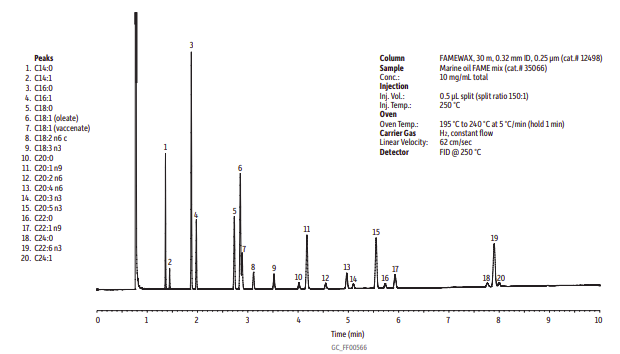
\includegraphics[width=12.5cm]{chromatograph.png}
  \caption{
    Gas chromatograph: the artifact of the GC method \cite{restek2018high}.
    The detection is used to visualize intensity (y) and time (x) on a chromotrogaph.}
  \label{fig:gas-chromatography} 
  \captionsetup[figure]{font=small,labelfont=small}
\end{figure}

Figure~\ref{fig:gas-chromatography} shows a gas chromatograph, chemists use the chromatagraphs for known reference samples to classify unknown samples. 
Analysis can identify unknown compounds since they share the same peaks to the known one.
GC is not a definitive technique \cite{khan2013gas}, so it is often used in conjunction with other techniques like Mass spectrometry \cite{restek2018high}.

The existing task of classifying chemical compounds based on a chromatograph is laborious \cite{eder1995gas,restek2018high}.
The spikes on the graph represent peaks.
Each peak represents a resolved chemical compound.
Chemists integrate the area under each peak, and compare this to a reference sample, to classify the compound.
GC must be performed slowly to ensure that the peaks are not too broad.
This ensures each peak resolves and represents a single compound.
Once we know what compounds are present in a sample it becomes possible to identify what the sample is.
For this fish oil data, we classify a sample into two categories - species and part. 

\subsection{Feature Selection}
\label{sec:background-feature-selection}

% TODO [ ] - This section needs to have more descriptions, including general ideas, that algorithms I will use in this work. 

Feature selection reduces the complexity of the problem space.
This helps counteract the curse of dimensionality \cite{koppen2000curse}.
Reducing the complexity improves computational efficiency, increases interpretability, and can improve performance.
More interpretable models are easier for humans to understand.
This means we can verify their efficiency using domain expertise in biochemistry.
This is an important factor for real-world applications in a factory setting.

\begin{enumerate}
  \item Chi$^2$ \cite{liu1995chi2}
  \item Minimum Redundancy Maximum Relevance \cite{ding2005minimum}
  \item ReliefF \cite{robnik2003theoretical}
  \item Particle Swarm Optimization \cite{kennedy1995particle,kennedy1997discrete}
\end{enumerate}

Liu et al. proposed Chi2 \cite{liu1995chi2}, a feature selection method via discretization. 
The algorithm is a generalized version of ChiMerge \cite{kerber1992chimerge} that determine a good $\Chi^2$ threshold automatically from the data.
The technique performs both feature selection and discretiszation, making it ideal for continious numeric fish oil data. 
The method can increase predictive perofrmance, efficiency (time/memory) and simplify models. 

\section{Data processing}

% TODO [ ] - Bach to fill out these sections. 

\begin{itemize}
  \item Why the raw data is not applicable to existing classification algorithms?
  \item Extracting datasets that are ready for classification algorithms:
        \begin{itemize}
          \item Sum up the intensity.
          \item Aligning missing packets.
        \end{itemize}
  \item Overview of extracted data.
\end{itemize}

\section{Classification}

We measure the predictive ability of classifiers on both the fish species and part dataset.
We are looking for the model with the highest accuracy.
As a result, we start broadly by exploring a variety of models from the different families of AI, and then we narrow and refine the search.
\\\\
For each of the following experiments, the same experiment setup is used.
We use stratified cross-validation ($k=10$) to measure the classification accuracy.
Each method has its performance recorded on the same cross-folds.
Then we average over 30 independent runs.
This experimental setup evaluates performance on both the fish species and part datasets.

\subsection{Classification Algorithms}

% TODO [ ] - Overal steps 
% 1. How do you perform classification here? 
% 2. Splitting the data? 
% 3. Training/test? 
% 4. 10-fold cross-validation? 
% 5. Why 30 independent runs? 

% This is a broad search for an effective classification model.
% We explore a classifier from each family of AI.
% The model with the highest classification accuracy on both datasets is then selected, and explored in later sections in further detail.

% TODO [ ] - Provide a short description for each algorithm here! What are there parameter settings? 
% TODO [ ] - Why KNN and NB have std != 0, these are deterministic methods. 

We examine 5 classification models:

\begin{enumerate}
  \item K-Nearest Neighbors \cite{fix1989discriminatory}
  \item Random Forest \cite{ho1995random}
  \item Naive Bayes \cite{hand2001idiot}
  \item Decision Tree \cite{loh2011classification}
  \item Support Vector Machine \cite{cortes1995support}
\end{enumerate}

\begin{table}[htb]
  \captionsetup{font=small,labelfont=small}
  \centering
  \begin{tabular}{|l|l|l|l|l|}
    \hline
    Dataset                    & Method & 
    AvgTrain $\pm$ Std         & 
    % T                          &
    AveTest $\pm$ Std                      \\ % &
    % T                                     \\
    \hline
    Species                    & 
    \begin{tabular}[c]{@{}l@{}}
      KNN          \\ % K-Nearest Neighbors
      RF           \\ % Random Forest
      DT           \\ % Decision Tree
      NB           \\ % Naive Bayes
      \textbf{SVM} \\ % Support Vector Machine
    \end{tabular} & 
    \begin{tabular}[c]{@{}l@{}}
      83.57 $\pm$ 1.80         \\ % KNN
      1.00 $\pm$ 0.00          \\ % RF
      1.00 $\pm$ 0.00          \\ % DT
      79.54 $\pm$ 1.60         \\ % NB
      \textbf{1.00 $\pm$ 0.00} \\ % SVM
    \end{tabular} & 
    \begin{tabular}[c]{@{}l@{}}
      74.88 $\pm$ 12.54          \\ % KNN
      85.65 $\pm$ 10.76          \\ % RF
      76.98 $\pm$ 13.12          \\ % DT
      75.27 $\pm$ 4.35           \\ % NB
      \textbf{98.33 $\pm$ 5.00 } \\ % SVM
    \end{tabular}             \\
    \hline
    Part                       & 
    \begin{tabular}[c]{@{}l@{}}
      KNN          \\ % K-Nearest Neighbors
      RF           \\ % Random Forest
      DT           \\ % Decision Tree
      NB           \\ % Naive Bayes
      \textbf{SVM} \\ % Support Vector Machine
    \end{tabular} & 
    \begin{tabular}[c]{@{}l@{}}
      68.95 $\pm$ 3.49          \\ % KNN
      1.00 $\pm$ 0.00           \\ % RF
      1.00 $\pm$ 0.00           \\ % DT
      65.54 $\pm$ 2.69          \\ % NB
      \textbf{1.00 $\pm$ 0.00 } \\ % SVM
    \end{tabular} & 
    \begin{tabular}[c]{@{}l@{}}
      43.61 $\pm$ 13.48          \\ % KNN
      72.60 $\pm$ 16.15          \\ % RF
      60.14 $\pm$ 14.57          \\ % DT
      48.61 $\pm$ 12.19          \\ % NB
      \textbf{87.14 $\pm$ 8.52 } \\ % SVM
    \end{tabular}             \\
    \hline
  \end{tabular}
  \caption{
    Accuracy for different classification techniques.
    Accuracy is given as the stratified k-fold cross validation over 30 independent runs.
    % We compare K-nearest neighbours (KNN), random forest (RF), decision tree (DT), naive bayes (NB) and support vector machines (SVM).
    }
  \label{t:classification}
\end{table}

Table~\ref{t:classification} shows for the random forest, decision tree and support vector machine have perfect training accuracy.
The decision tree and random forest overfit the training data.
Only the SVM achieves similar performance on the test data.
The SVM classifier outperforms the other classifiers.
It does so for the test set for both the species and part datasets.

% TODO [ ] More analysis needed here? 
% 1. Should compare algorithms performance based on number, e.g. SVM is 20% more accurate than KNN, DT, and NB. 
% 2. Why NB and KNN do not work well? Why DT overfits the data (you use full size)? RF is better because of ensemble mechanism? Too many features too few instances? 

\subsection{Discussion}
\label{sec:results-classification-discussion}

We evaluated an ensemble of classification techniques.
Naive Bayes performed poorly.
This is likely due to the assumption of conditional independence between features.
KNN also performed poorly. This is likely due to the high dimensionality of the data.
Points drawn from high-dimensional spaces tend to never be close together.
SVM provided the best results.
This model can identify fish species from gas chromatography data with near-perfect accuracy.
This prompted further investigation into this technique.

Classification accuracy for all models was better for the fish species than the part.
This suggests tissue samples for different species may have distinct chemical compositions.
Yet, different fish parts may have fewer underlying structural differences.
For GC data the intra-class variation between species provides a larger signal than part variation.
For example, we expect there to be more difference between a tarakihi and a bluecod, than there is a similarity between two livers from different species.

\subsection{Weight Analysis}

% TODO [] - Replace 4.2 and 4.3 by weight analysis.
% It is good that you perform different settings for SVM, but I doubt these additions would increase the paper's value. 
% I remember you did analyse the weight vectors of the model to give an overview of some features may not be used. Such analysis is more valuable
% TODO [ ] Motivation for FS - It is also a good motivation for feature selection.

\subsubsection{Visualisation}
\label{sec:visualisation}

% TODO [ ] - This part can be shortened, and included in the visualisation sections, (not background)

Two heuristics are optimized when selecting a suitable model: interpretability and accuracy. 
Interpretability is important for verification in a safety-critical environment.
We intend to employ the chosen model in a factory setting.
Accuracy is preferable, but not at the expense of interpretability.
The efficacy of the model must be explainable through domain knowledge.
Or else it is difficult to ensure reliability.
The focus on interpretability ensures the model can be used in the real world.

Model interpretability is explored through visualisation.
We aim to uncover learnt patterns that can be verified with domain knowledge.
The desired algorithm should strike a balance between predictive performance and semantically meaningful features.

What constitutes semantic meaning varies from one domain to another.
It is easy to build intuition for semantic meaning in computer vision and natural language processes, they correspond to recognisable images and structured text.
In the domains of gas chromatography and fish processing, our meaning is derived from performance on the classification task(s) and similarity to underlying chemical compounds.
We expect models that generate knowledge that can be verified with domain expertise. 
For example, important features will correspond to timestamps of important chemicals in the GC data.

% TODO [ ] - This part can be removed, a brief description can be provided when SVM is used. 
% TODO [ ] - Other classification algorithms, describe each of these later, when used. 

\subsubsection{SVM Hyperplane Coefficients}

Cortes and Vapnik proposed the Support Vector Machine (SVM) \cite{cortes1995support}.
This model creates a hyperplane that can draw distinct class boundaries between classes.
We call these class boundaries the support vectors.
We are performing multi-class classification, so it used a one-vs-all approach \cite{sklearn2021feature}.
This creates a divide between one class and the rest, then repeats for the other classes.

The l1 regularization term leads to sparse models.
So, they include fewer features - making them easier to interpret.
Eq~\ref{eq:hyperplane} defines the total hyperplane as

\begin{align}\label{eq:hyperplane}
  \beta_{\text{t}} = \text{minmax}(
  \sum_{\text{c} \in \text{C}}
  |\beta_{\text{c}}|
  )
\end{align}

where there is the number of classes ($c \in C$) sets of hyperplane coefficients.
$\beta_{\text{t}}$ coefficient as the sum of hyperplane coefficients magnitude for each class $\beta_{\text{c}}$.
We normalize the coefficients with a min-max feature scaling.

\begin{figure}[htb]
  \centering  
  \begin{subfigure}[b]{.55\linewidth}
    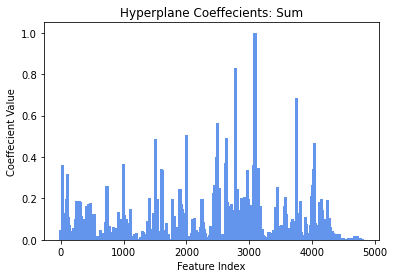
\includegraphics[width=\linewidth]{fish_total_coefficients.png}
    \caption{Fish Species: Hyperplane Coefficients}\label{fig:fish-hyperplane-coeffcients}
  \end{subfigure}
  \begin{subfigure}[b]{.55\linewidth}
    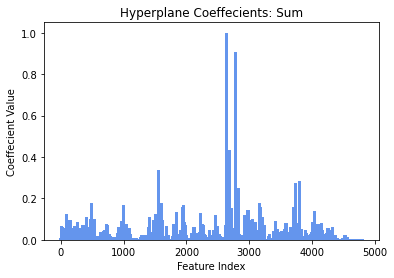
\includegraphics[width=\linewidth]{part_total_coefficients.png}
    \caption{Fish Part: Hyperplane Coefficients}\label{fig:part-hyperplane-coeffcients}
  \end{subfigure}
  \caption[Two numerical solutions]{
    Hyperplane coefficients $\beta_t$.
    The normalized sum of the magnitude of the coefficients for each class is given in Eq~\ref{eq:hyperplane}.
    (a) Coefficients for the fish species dataset.
    (b) Coefficients for the fish part dataset.}
  \label{fig:hyperplane-coefficients}
\end{figure} 

The total hyperplane for both datasets is given in Figure~\ref{fig:hyperplane-coefficients}.
We visualize the hyperplane to approximate the important features. 
The outliers correspond to feature timestamps that are important for drawing class boundaries. 
These are chemical compounds that separate the fish part and species, respectively. 

\section{Feature Selection}

% TODO [ ] - Why feature selection on this data?
% TODO [ ] - Brief the main ideas of the feature selection algorithms that were used.

\begin{itemize}
  \item Why feature selection on this data? 
  \item Brief the main ideas of the feature selection algorithms that were used. 
\end{itemize}

For each method, we measure classification accuracy with an SVM model \cite{sklearn2021feature}.
It has linear kernel, l1 regularization \cite{robnik2003theoretical} and 10,000 maximum iterations.
We examine 4 feature selection methods \cite{chappers2015skfeature}:

\begin{enumerate}
  \item Chi$^2$ \cite{liu1995chi2}
  \item Minimum Redundancy Maximum Relevance \cite{ding2005minimum}
  \item ReliefF \cite{robnik2003theoretical}
  \item Particle Swarm Optimization \cite{kennedy1995particle,kennedy1997discrete}
\end{enumerate}

We measure classification accuracy as a function of feature number.
We compared this for several FS methods.
Due to limitations, PSO optimizes feature number $k$ automatically.
So, to compare its performance, we plot the results of 30 independent runs.
\\\\

% TODO [ ] Fix the figures. 
% 1. Enlarge the font on the figures. 
% 2. Make sure the algorithm names in the legend is the same as in the paragraph. 
% [x] 3. You can have 2 different graphs for fish species and part. 

\subsection{Fish Species}

\begin{figure}[htb]
  \centering
  \begin{subfigure}[b]{.55\linewidth}
    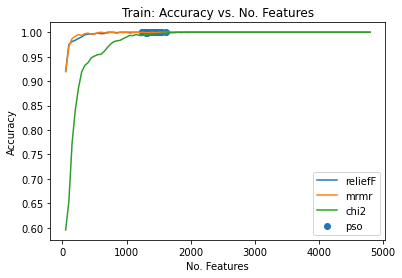
\includegraphics[width=\linewidth]{accuracy-features-fish-train.png}
    \caption{Species: Training set}\label{fig:accuracy-features-fish-train}
  \end{subfigure}
  \begin{subfigure}[b]{.55\linewidth}
    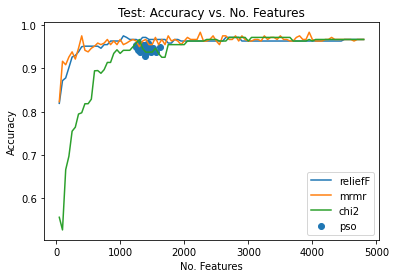
\includegraphics[width=\linewidth]{accuracy-features-fish-test.png}
    \caption{Species: Test set}\label{fig:accuracy-features-fish-test}
  \end{subfigure}
  \caption[Two numerical solutions]{
    Fish species dataset: Classification accuracy for feature selection methods for a given $k$.
    We measure the balanced accuracy of k-fold cross-validation.
    We compare reliefF, maximum relevance - minimum redundancy (MRMR), chi$^2$, and particle swarm optimisation (PSO).
    Fish part dataset. (a) Training set. (b) Test set.}
  \label{fig:animals}
\end{figure}

Figure~\ref{fig:accuracy-features-fish-train} shows accuracy for fish species.
We show accuracy on the training set for each feature selection method.
At $k=1050$ all feature selection methods achieve $100\%$ accuracy on the training set.
The SVM fits the training data for each method using a fraction of the full feature set.
Figure~\ref{fig:accuracy-features-fish-test} shows accuracy for fish species.
We show test set accuracy for each feature selection method.
The accuracy reaches a plateau ($96\%$ accuracy) at around $k=1050$ features for all methods.
The test performance is less than the train performance, yet the test accuracy is still very high.
This suggests the model can generalize well on unseen data for the fish species.

\subsection{Fish Part}

\begin{figure}[htb]
  \centering
  \begin{subfigure}[b]{.55\linewidth}
    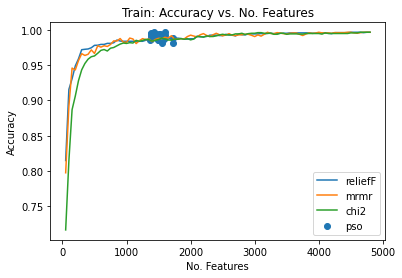
\includegraphics[width=\linewidth]{accuracy-features-part-train.png}
    \caption{Part: Training set}\label{fig:accuracy-features-part-train}
  \end{subfigure}
  \begin{subfigure}[b]{.55\linewidth}
    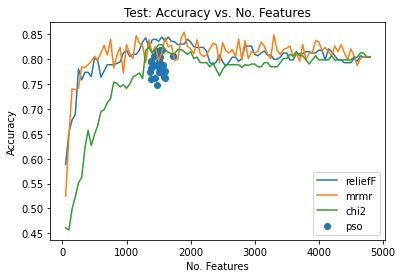
\includegraphics[width=\linewidth]{accuracy-features-part-test.png}
    \caption{Part: Test set}\label{fig:accuracy-features-part-test}
  \end{subfigure}
  \caption[Two numerical solutions]{
    Fish part dataset: classification accuracy for feature selection methods for a given $k$.
    We measure the balanced accuracy of k-fold cross-validation.
    We compare reliefF, maximum relevance - minimum redundancy (MRMR), chi$^2$, and particle swarm optimisation (PSO).
    Fish part dataset. (a) Training set. (b) Test set.}
  \label{fig:accuracy-features-part-train}
\end{figure}

Figure~\ref{fig:accuracy-features-part-train} shows accuracy for part dataset.
We show train accuracy for each feature selection method.
All feature selection methods struggle to fit the training set for the fish part.
Even with the full feature set, a perfect train accuracy is never reached.
Figure~\ref{fig:accuracy-features-part-test} shows accuracy for part dataset.
We show the test accuracy for each feature selection method.
The classification accuracy fluctuates for all feature selection methods.
At around $k=1050$ features, it begins to decrease.
The training accuracy improves, as the test does not from this point onwards.
The SVM is overfitting to noise (redundant features) in the training set.

% TODO [ ] - Compare the performance of selected features and use all features.
% TODO [ ] - (Optional): analyse the selected features.

\begin{itemize}
  \item Compare the performance of selected feautres and use all feautres. 
  \item (Optional) analyse the selected features .
\end{itemize}

% TODO [ ] - Rewrite all. Which algorithms work best on the species data. 
% TODO [ ] - Discussion on different algorithms. 
% 1. PSO achieves the best trainign accuracies with much smaller number fo features. 
% 2. Testing accuraces of PSO are not that good, potential overfitting, future work. 
% 3. Other algorityhms also achieve best performance at around 1050 feautres, FS is helpful to imrpove the part classification. 

\subsection{Disucssion}
\label{sec:results-feature-selection-discussion}

% TODO [ ] - Move 
% This discussion can be provided right after the results discussion. 

Feature selection methods helped reduce dimensionality.
We evaluated performance with an SVM classifier.
Which, ReliefF and PSO were best for fish species and part, respectively.
ReliefF can identify conditional dependencies between features when providing feature rankings.
ReliefF algorithms are robust and noise-tolerant, which explains their superior performance.
PSO provides a combination of global and local searches.
A search through a near-infinite combinatorial space of possible feature subsets.
This stochastic method is computationally expensive but can offer effective solutions.

% TODO [ ] Remove - reported in the classification part. 
For both general and specific cases, and across all methods, the fish species have lower variance than the fish part in classification accuracy.
The classification results support this, they also show higher test accuracy for fish species, than for fish parts.
They suggest different fish parts may have fewer underlying structural differences.

% TODO [ ] Remove - Already discussed previously. 
For the general case and both datasets, a lot of interesting behaviour happens at $k=1050$.
The fish species reach a plateau, but the fish part accuracy begins to decrease.
Accuracy comparable to or better than the full dataset is possible with 21.8\% of its features.

% TODO [ ] Trim - some ideas have already been discussed, extend Bach's comments into full paragraphs instead. 
For the fish species dataset, we see high accuracy with very few features.
ReliefF and MRMR can achieve above 90\% classification accuracy with $k = 50$.
Chi$^2$ is not able to mirror this performance.
This shows that ReliefF and MRMR are very effective feature selection methods for this task.

The PSO may not have a hyperparameter for feature number $k$.
Instead, it automates the selection of this parameter.
Yet, it achieves comparable results to other state-of-the-art methods.
This automation may prove useful for automating the classification task for online learning.
In a factory, we may want to train a model as new data arrives.
PSO requires less human intervention, yet still, provides competitive performance.

MRMR and ReliefF both have high accuracy with very few features on the fish species dataset.
This suggests that few features are required to construct a reasonable representation of a fish tissue sample.
This is a good indication that the fish species dataset contains less noise.
% This also warrants further investigation into which features are considered important for low $k$ values.
% This motivates the following section on visualisation.

\section{Conclusions and Future Work}

% TODO [ ] Visualistion - I found no visualisation and interpretable models in this paper? 
This paper has demonstrated an interpretable and effective method for fish oil analysis. 
The method can be understood, domain experts can understand the important features in the decision-making.
Not only have we found effective classification and feature selection techniques, but we have also tried to explain their performance with visualisation and analytical results. 
We can draw many conclusions from the analytical results and visualisations, but here we recall the most important:

\begin{enumerate}
  \item Fish species are easier to predict than fish parts - there is more intra-class variation within fish species than there is a similarity between the same part from different fish.
  \item The Linear SVM classifier performs better for both classification tasks - the fish oil data is linearly separable on a hyperplane.
  \item This model can achieve 90\% fish species accuracy using only 1\% (k = 50) of its features, enabling efficient training, and showing many redundant features. 
  % TODO [ ] - Add the weight analysis 
\end{enumerate}

LinearSVC applied to GC fish oil data can help to reduce waste in fish processing. 
This ensures more sustainable eco-friendly practices in fish processing.
Waste reduction and repurposing is a rising tide that lifts all boats.
Sustainable practices will leave plenty of fish in the sea, preserving resources for future generations. 

% TODO [ ] - Future work: further steps, improve fish part performance, more challenging datasets, different tasks. 

% Please note that the first paragraph of a section or subsection is
% not indented. The first paragraph that follows a table, figure,
% equation etc. does not need an indent, either.

% Subsequent paragraphs, however, are indented.

% \subsubsection{Sample Heading (Third Level)} Only two levels of
% headings should be numbered. Lower level headings remain unnumbered;
% they are formatted as run-in headings.

% \paragraph{Sample Heading (Fourth Level)}
% The contribution should contain no more than four levels of
% headings. Table~\ref{tab1} gives a summary of all heading levels.

% \begin{table}
% \caption{Table captions should be placed above the
% tables.}\label{tab1}
% \begin{tabular}{|l|l|l|}
% \hline
% Heading level &  Example & Font size and style\\
% \hline
% Title (centered) &  {\Large\bfseries Lecture Notes} & 14 point, bold\\
% 1st-level heading &  {\large\bfseries 1 Introduction} & 12 point, bold\\
% 2nd-level heading & {\bfseries 2.1 Printing Area} & 10 point, bold\\
% 3rd-level heading & {\bfseries Run-in Heading in Bold.} Text follows & 10 point, bold\\
% 4th-level heading & {\itshape Lowest Level Heading.} Text follows & 10 point, italic\\
% \hline
% \end{tabular}
% \end{table}


% \noindent Displayed equations are centered and set on a separate
% line.
% \begin{equation}
% x + y = z
% \end{equation}
% Please try to avoid rasterized images for line-art diagrams and
% schemas. Whenever possible, use vector graphics instead (see
% Fig.~\ref{fig1}).

% \begin{figure}
% 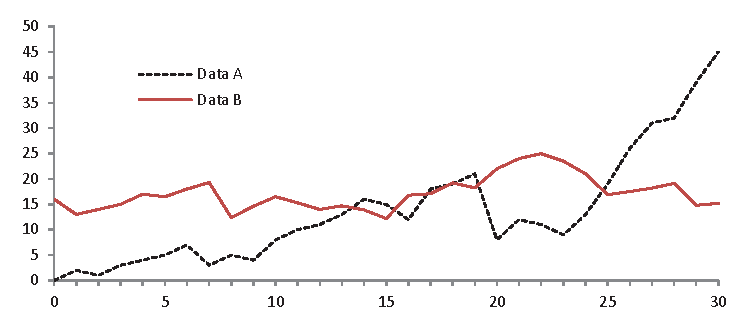
\includegraphics[width=\textwidth]{fig1.eps}
% \caption{A figure caption is always placed below the illustration.
% Please note that short captions are centered, while long ones are
% justified by the macro package automatically.} \label{fig1}
% \end{figure}

% \begin{theorem}
% This is a sampling theorem. The run-in heading is set in bold, while
% the following text appears in italics. Definitions, lemmas,
% propositions, and corollaries are styled the same way.
% \end{theorem}
%
% the environments 'definition', 'lemma', 'proposition', 'corollary',
% 'remark', and 'example' are defined in the LLNCS documentclass as well.
%
% \begin{proof}
% Proofs, examples, and remarks have the initial word in italics,
% while the following text appears in normal font.
% \end{proof}
% For citations of references, we prefer the use of square brackets
% and consecutive numbers. Citations using labels or the author/year
% convention are also acceptable. The following bibliography provides
% a sample reference list with entries for journal
% articles~\cite{ref_article1}, an LNCS chapter~\cite{ref_lncs1}, a
% book~\cite{ref_book1}, proceedings without editors~\cite{ref_proc1},
% and a homepage~\cite{ref_url1}. Multiple citations are grouped
% \cite{ref_article1,ref_lncs1,ref_book1},
% \cite{ref_article1,ref_book1,ref_proc1,ref_url1}.
%
% ---- Bibliography ----
%
% BibTeX users should specify bibliography style 'splncs04'.
% References will then be sorted and formatted in the correct style.
%
\bibliographystyle{splncs04}
% \bibliography{mybibliography}
\bibliography{refs}

\end{document}
